\documentclass[a4paper,11pt]{article}
\usepackage{lecturenotes}
\usepackage{caption}
\lectureheader{ELE745}{2}
\begin{document}
\notesection{Formatting and Digital Coding of Waveforms}
The original form of most communicated data is either textual or analog, and needs to be converted to binary bits for transmission

\subnotesection{Sampling}
\notedefinition{Sampling Theorem}{A signal with maximum frequency $f_m$ requires $f_s \geq 2f_m$ samples/s.}

In practice, sampling multiplies $x(t)$ by the impulse train $x_\delta(t)$, whose pulses are separated by the sampling period $T_s$:

\begin{notederivation}{Sampled Signal Formula}
    \setlength{\jot}{2pt}%
    & x_\delta(t) = \sum_{n=-\infty}^{\infty} \delta(t-nT_s) && \qquad \text{Definition of Pulse Train} \\
    & D_{n, \delta} = \frac{1}{T_s}\int_{-T_s/2}^{T_s/2} x_p(t)e^{-jn2\pi f_s t} dt = 1/T_s && \qquad \text{Fourier Series of Pulse Train} \\
    & X_{\delta}(f) = \frac{1}{T_s}\sum_{n=-\infty}^{\infty} \delta(f-nf_s) && \qquad \text{Fourier Transform of Pulse Train} \\ 
    & x_s = x(t) \cdot x_\delta(t) = \sum_{n=-\infty}^{\infty} x(t) \cdot \delta(t-nT_s) = \sum_{n=-\infty}^\infty x(nT_s)\delta(t-nT_s) && \qquad \text{Time Domain Representation} \\
    & X_s(f) = X(f) * X_\delta(f) = \frac{1}{T_s}\sum_{n=-\infty}^{\infty}X(f-nf_s) && \qquad \text{Frequency Domain Representation}
\end{notederivation}

\keyequation{Sampled Signal Representations}{
    \begin{aligned}
        x_s(t) &= \sum_{n=-\infty}^\infty x(nT_s)\delta(t-nT_s), \quad X_s(f) &= \frac{1}{T_s}\sum_{n=-\infty}^{\infty}X(f-nf_s)
    \end{aligned}
}
\begin{itemize}
    \setlength{\topsep}{2pt}
    \setlength{\itemsep}{0pt}
    \item $X_s(f)$ is a periodic function of the original spectrum scaled by a constant factor and centered at $nf_s$
    \item Aliasing will occur if sampling frequency is not high enough
\end{itemize}
\enlargethispage{2\baselineskip}
\begingroup
    \captionsetup{font=footnotesize,skip=3pt}
    \noindent
    \begin{minipage}[t]{0.46\linewidth}
        \centering
        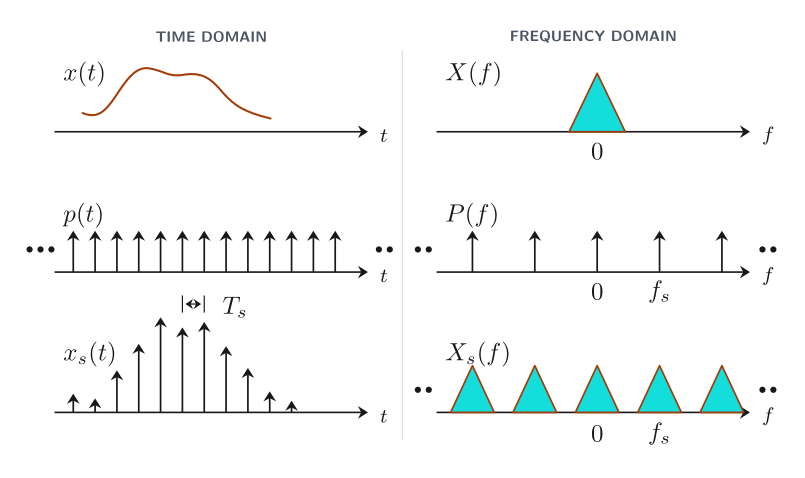
\includegraphics[width=\linewidth]{figures/sampling_time_frequency_diagram.png}
        \captionof{figure}{Sampling in the time and frequency domains.}
        \label{fig:sampling-time-frequency}
    \end{minipage}\hfill
    \begin{minipage}[t]{0.46\linewidth}
        \centering
        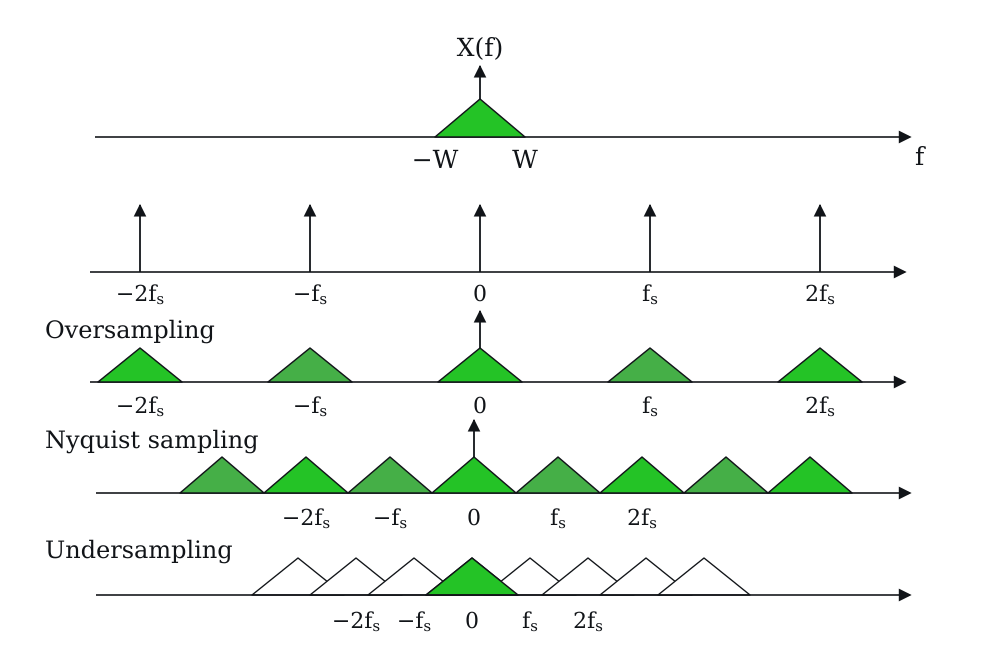
\includegraphics[width=\linewidth]{figures/sampling_regimes_frequency_spectra.png}
        \captionof{figure}{Spectral replicas for oversampling, Nyquist sampling, and undersampling.}
        \label{fig:sampling-regimes}
    \end{minipage}
\endgroup

\subnotesection{Ideal Signal Reconstruction}
Recall the spectrum of the sampled signal, we can then recover the signal as:
$$
X(f) = \frac{1}{f_s}X_s(f)\cdot \operatorname{rect}\!\left(\frac{f}{2B}\right)
$$

Where: $\operatorname{rect}\!\left(\frac{f}{2B}\right)=\begin{cases}
    1 & -B\leq f \leq B \\
    0 & \text{o.w}
\end{cases}
$

\begin{notederivation}{Time-Domain Representation of Ideal Signal Recovery}
    & x(t) = \mathcal{F}^{-1}[X(f)]
        = \frac{1}{f_s}\mathcal{F}^{-1}\!\left[X_s(f)\cdot\operatorname{rect}\!\left(\frac{f}{2B}\right)\right]
        && \qquad \text{Ideal low-pass filtering} \\
    & \phantom{x(t)} = \frac{1}{f_s}\mathcal{F}^{-1}[X_s(f)]
        * \mathcal{F}^{-1}\!\left[\operatorname{rect}\!\left(\frac{f}{2B}\right)\right]
        && \qquad \text{Convolution theorem} \\
    & \phantom{x(t)} = \frac{1}{f_s}x_s(t)*\bigl(2B\,\operatorname{sinc}(2\pi Bt)\bigr)
        = \frac{2B}{f_s}x_s(t)*\operatorname{sinc}(2\pi Bt)
        && \qquad \text{Inverse transform pair} \\
    & \phantom{x(t)} = \frac{2B}{f_s}\left[\sum_{n=-\infty}^{\infty}x(nT_s)\delta(t-nT_s)\right]
        * \operatorname{sinc}(2\pi Bt)
        && \qquad \text{Substitute sampled signal} \\
    & \phantom{x(t)} = \frac{2B}{f_s}\sum_{n=-\infty}^{\infty}x(nT_s)\,
        \operatorname{sinc}\!\bigl(2\pi B(t-nT_s)\bigr)
        && \qquad \text{Sinc interpolation}
\end{notederivation}
If $f_s = 2B$ then:
\keyequation{Interpolation Formula for Signal Reconstruction}{x(t) = \sum_{n=-\infty}^{\infty}x(nT_s)\cdot \operatorname{sinc}\Big[ 2\pi B (t-nT_s)\Big]}

\subnotesection{Practical Sampling}
In reality however, the actual sampling signal is defined as: $c(t) \frac{A_\tau}{T_s}\sum_{n=-\infty}^\infty \operatorname{sinc}(n\pi f_s \tau)e^{j2\pi n f_s t}$.
\keyequation{Practical Sampling Sampled Signal Equation}{
    \begin{aligned}
        x_s(t) &= \frac{A_\tau}{T_s} \cdot x(t) \sum_{n=-\infty}^{\infty} \operatorname{sinc}(n\pi f_s \tau)e^{j2\pi n f_s t} \\
        X_s(f) &= \frac{A_\tau}{T_s} \sum_{n=-\infty}^{\infty} \operatorname{sinc}(n\pi f_s \tau) \cdot X(f-nf_s)
    \end{aligned}
}
During natural sampling we observe that \textbf{A)} No distortion in recieving $x(t)$ if $f_s > 2B$ and \textbf{B)} if $A\tau = 1$, natural sampling is equivalent to ideal sampling when $n=0$

\begin{figure}[htbp]
    \centering
    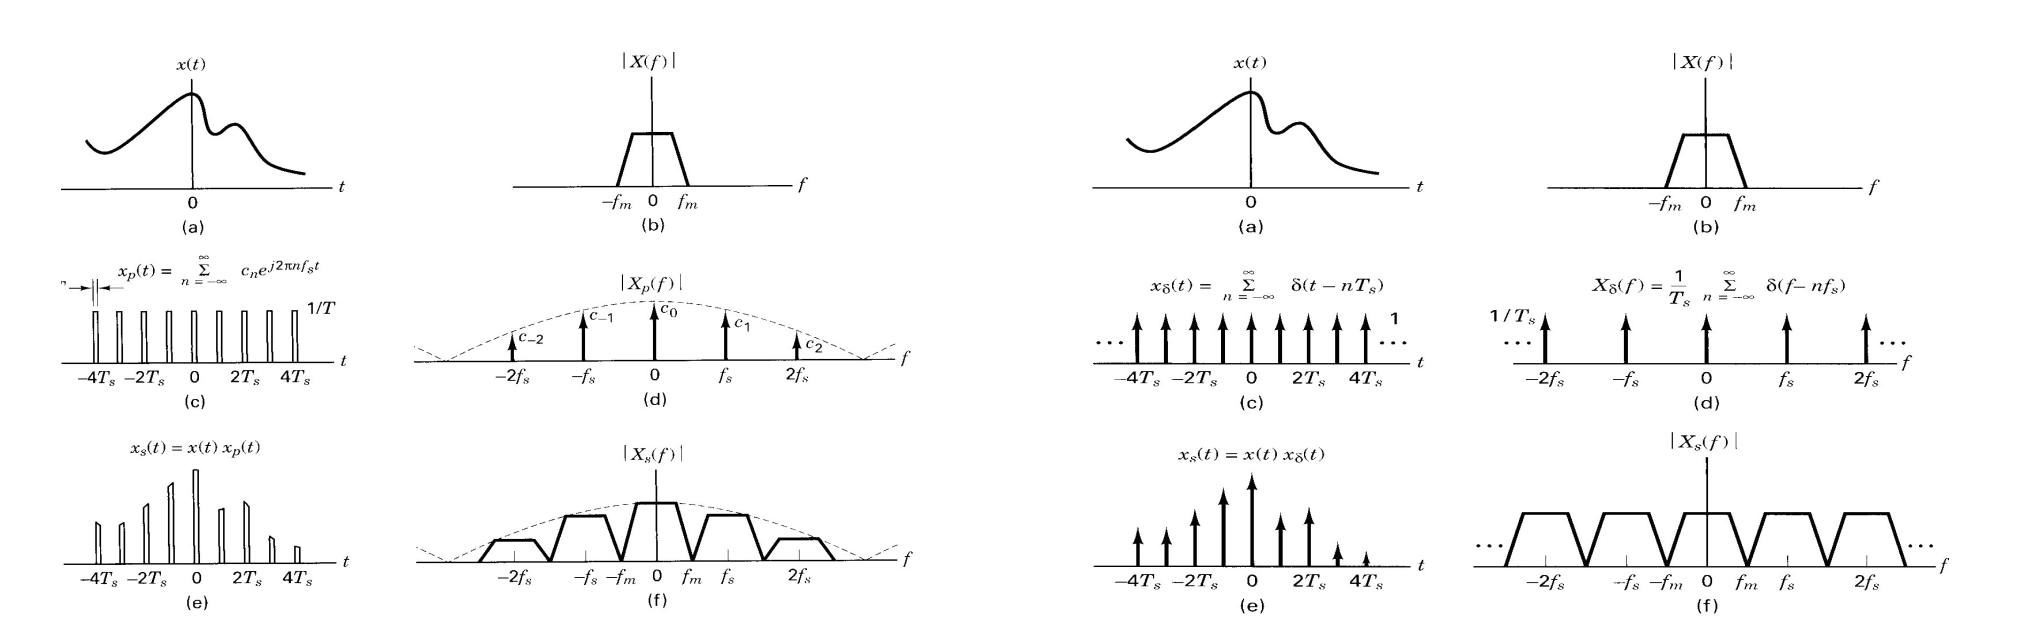
\includegraphics[width=0.8\linewidth]{figures/natural_and_ideal_sampling.png}
    \caption{Natural and Ideal Sampling}
    \label{fig:}
\end{figure}

\notesection{Quantization}
Process in which the amplitude of the sampled signal (discrete-time) is limited to a pre-defined set of new voltage levels. Introducing a quantization error, $e(t)$, for each sample.
\notedefinition{Quantization Error}{$e = x_q - x_s$}

\keyequation{E as a Random Variable with Uniform Distribution}{
    e = x_q - x_s
}[\begin{itemize}
    \item Stepsize: $q = \frac{V_{pp}}{L}$
    \item Quantization Levels: $L=2^N$
    \item Quantization Bits: N
    \item Range: $-\frac{q}{2}\geq e \geq \frac{q}{2}$
\end{itemize}]

\keyequation{Probability Density Function (PDF) of Quantization Error}{f(e) = \begin{cases}
    \frac{1}{q} & -\frac{q}{2}\geq e \geq \frac{q}{2} \\
    0 & \text{otherwise}
\end{cases}}

\keyequation{Quantization Noise Power}{\sigma^2_q = E[e^2] = \frac{q^2}{12}}
\keyequation{Signal Noise Power}{\operatorname{SNR} = \frac{P_{\text{signal}}}{\sigma^2}}
\notesection{PCM Modulation}

\end{document}
